% \section{Outline}

% \begin{enumerate}
%     \item Introduction
%     \begin{enumerate}
%         \item DNN workloads are valuable
%         \item Acceleration of DNNs is valuable
%         \item There are many ways of accelerating DNNs, software and hardware
%         \item Picking the right accelerator with the right hardware resources is dependent on the kernel
%         \item There are many different approaches to neural network-based solutions. (i) Some, such as HTM, are more biologically accurate, some are (ii) synthetic but still biologically inspired. As part of these approaches, there are many algorithms (kernels) in DNN, which are suited to different types of data, the most important kernels are CNN, LSTM, and MLP
%         \item The metrics of interest in accelerating these workloads are average turnaround time, i.e., latency, or number of inferences per second, i.e., throughput. System-level metrics include efficiency and utilization. These are the metrics by which we can compare between two accelerator implementations. 
%         \item There are many different accelerator options, with different parallel resources. Spatial architectures offer opportunities to parallelize DNN workloads because of their available ILP and TLP resources
%     \end{enumerate}
%     \item HTM on the AP
%     \begin{enumerate}
%         \item HTM is valuable because it is an attempt to distill the principles of the neocortex into software.
%     \end{enumerate}
%     \item Dissertation chapters
%     \begin{enumerate}
%         \item Mapping HTM to the AP
%         \item Automatic synthesis of HTM models on the AP
%         \item Mapping DNNs to systolic arrays
%         \item Optimization of DNN workloads on systolic arrays
%         \item 
%     \end{enumerate}
% \end{enumerate}

% \pagebreak
\section{Introduction}

Brain-inspired and ``cognitive''-style algorithms have become a critical part of computer software applications in the domains of classification, regression, anomaly detection, and prediction.
Rather than being explicitly programmed through static instructions, these algorithms are more brain-like than classical approaches, such as statistical methods, because they mimic the brain's capabilities for autonomous pattern learning and generalization by automatically building internal representations from exposure to data.
If we consider of the brain as the energy efficient ``hardware'' of mammalian intelligence~\cite{laughlin2003communication}, it is interesting to study the kinds of properties that the best hardware of \textit{silicon} intelligence might inherit from the brain, towards achieving comparable functionality and efficiency.

Artificial neural networks (ANNs)~\cite{mcculloch1943logical, hebb2005organization, farley1954simulation, rochester1956tests} are a broad class of machine learning algorithms that are inspired by both the structure and the functionality of biological neural networks, and are the basis of the majority of modern machine learning software applications.
ANNs are operated in two phases: during \textit{training}, the functionality of the network is iteratively improved through exposure to input data as the internal weights are updated to match known good outputs.
Then during \textit{inference}, the network is presented with a new set of inputs, the input data values are combined with the trained neuron weights in each layer in sequence until a vector of outputs is produced at the final layer.

% \textit{Structurally}, ANNs are modeled as interconnected computational units called neurons, which are collected into a cascade of layers.
% Neurons accept a vector of inputs that are combined with internal weight parameters to produce an output, which is passed on to the next layer of neurons, and so on, the result of which is communicated to higher levels within a software framework.
% \textit{Functionally}, they can be trained to provide classification, detection, or prediction functions for various data types, while automatically generalizing from past experience.

Classical neural networks, such as multilayer perceptrons (MLPs)~\cite{rosenblatt1961principles}, and more recently, convolutional neural networks (CNNs)~\cite{lecun1999object} are especially adept at autonomously extracting features and interpreting \textit{structural} data, such as images or other multidimensional signals.
Deep neural networks (DNNs), modeled after the brain's visual and auditory cortices, contain many tens or hundreds of ANN layers~\cite{lee2009convolutional, simonyan2014very, sermanet2013overfeat, szegedy2015going, krizhevsky2012imagenet}, and have been used extensively and successfully for many applications focused on this type of data.
% Image recognition and classification, cancer diagnosis, spam filtering, voice recognition, and controlling self-driving vehicles are just a subset of such applications deployed on platforms ranging from cloud services, to smartphones and autonomous vehicles~\cite{hannun2014deep, he2016deep, hinton2012deep, krizhevsky2012imagenet, li2016persona, silver2016mastering, jafari2016extraction, fridman2017autonomous}.

In contrast, a related class of ANNs, called recurrent neural networks (RNNs), are designed to perform inference on \textit{temporal} signals.
RNNs contain local storage and cyclical connections that combine elements of past inputs with current inputs to predict future inputs.
As an example, hierarchical temporal memory (HTM)~\cite{ahmad2015properties, mnatzaganian2017mathematical} is closely modeled after the neocortex, and can learn to predict future outputs and detect anomalies by exposure to a stream of incoming data.
A more mainstream RNN example is long-short term memory (LSTM), which is the main algorithm behind applications such as natural language processing and machine translation.

\subsection{Problem Definition}

Given that these kinds of algorithms are a critical part of important modern software applications, it is valuable to implement them in computer hardware in a scalable and efficient way.
Broadly, the challenge to be addressed by this work is to improve the performance of a broad class of machine learning workloads while simultaneously improving their efficiency.
To improve (i) \textit{performance}, the challenge is to recognize the parallelism exposed by these algorithms at design time, at multiple levels of abstraction, and to efficiently map the algorithm to the available parallel hardware resources, in such a way that utilization is maximized.
To improve (ii) \textit{efficiency}, the challenge is to exploit prior knowledge of the workload characteristics of the algorithms to minimize underutilized hardware resources.

To study this problem systematically, we divide it into a number of sub-problems:
% Across domains, while an interconnected neuronal structure is similar for several mainstream machine learning computational \textit{kernels}, the workload characteristics of the algorithms can vary greatly, which can have a big impact on performance\cn.

\paragraphHeading{RNN spatial architecture acceleration} RNNs are very valuable for a variety of applications, and it has been reported that they make up a majority of workloads in datacenters, and accelerating them would also be very valuable.
Spatial architectures are a class of computer processor that have been shown to work well for accelerating neural network kernels, because they provide several dimensions of parallel compute resources. 
However, works applying spatial architectures for acceleration of neural networks focus almost exclusively on CNNs.
Nobody has yet clearly identified RNN workload parameters, and how these could efficiently be mapped to spatial architectures.

\paragraphHeading{LSTM spatial architecture dataflow} LSTMs have been accelerated on spatial architectures, but a processing dataflow has not been introduced that can process all LSTM operations.
Acceleration of LSTMs has been demonstrated on specialized hardware, but only using neural network primitives, such as dense and sparse matrix operations, which require significant additional communication overhead to generate output\cn. 
An efficient dataflow would identify opportunities and exploit data reuse, local accumulation, and reduction of communication to improve performance and efficiency in area-constrained spatial architectures. 

\paragraphHeading{Optimization of RNN on reconfigurable SA} Given the development of dataflow and reconfigurable hardware, what is needed is an application of dataflow and hardware configuration co-optimization to improve the performance and utilization of RNNs on dynamically reconfigurable spatial architecture. 
What is needed is an approach for optimizing spatial architectures to the 
% However, an important distinction is that the dimensions of data structures and order of operations as part of these algorithms are known at design time, which can be exploited to build efficient accelerator hardware.

\paragraphHeading{Dynamic hardware configuration} Optimization of general neural networks on spatial architectures has primarily been done at the software level, using dataflow optimization, leaving performance and efficiency margins unclaimed due to inefficient mapping to static architectures.
What is needed is a methodology that exploits the diversity in the computational characteristics among heterogeneous DNN layers to improve the energy efficiency of spatial architecture accelerators by dynamically configuring accelerator microarchitectural parameters.

% A high degree of data parallelism is a common characteristic among these kernels, which can be exploited to improve performance using computer architectures with many parallel resources.
% Because of the parallel nature of these algorithms, people have been successful with mapping these algorithms to highly parallel computer architectures.

% There are several key challenges within the context of accelerating neural network workloads in computer architectures.
% Doing this in an efficient way requires (i) recognizing similarities across DNN workloads that can be exploited to minimize logic overhead and (ii) recognizing inter-kernel differences and (iii) being able to adapt to intra-kernel differences, i.e., the dynamic characteristics across program phases. 

% There are many different ways to do this, the most popular being optimizing the dataflow, i.e., the mapping of the algorithm onto available hardware.
% While this is an important step in the optimization process, even the best dataflow leaves performance margins and underutilizes hardware\cn.

% Although the most common operations in DNNs have benefited from exploitation of SIMD and SIMT processing, there remain challenges to simultaneously meeting both performance and efficiency goals for these platforms.
% On CPU, dataflow optimizations and SIMD ISA extentions can be used to capture speedups over SISD, but this is  limited by the relatively small number of available compute units, and dynamic memory requirements that stress the cache hierarchy~\cite{vanhoucke2011improving}.
% GPUs provide very wide SIMD capabilities, and can provide deeper loop unrolling and more opportunity for hiding the latency of memory for large blocks of input data.
% However, thread divergence can cause significant reduction in utilization, especially in networks with many layers with heterogeneous workload characteristics, such as DNNs~\cite{hill2017deftnn}.
% Furthermore, they require large batching and while they improve throughput, their impact on latency is limited~\cite{jouppi2017datacenter}.
% Reconfigurable logic architectures for accelerating machine learning have also been proposed in FPGA substrates~\cite{putnam2014reconfigurable, ovtcharov2015accelerating, caulfield2016cloudscale, chung2017accelerating}.

% Several customized spatial architectures have been proposed for the acceleration of neural networks~\cite{chen2017eyeriss, han2016eie}.
% These spatial architectures have been shown to be the most promising, because they are able to take advantage of available opportunities for data reuse in DNN kernels to both improve performance and save power.
% While these have shown significant improvements in both performance and efficiency, all have focused on optimizing for fully-connected and convolutional kernels.
% Recent studies showing that recurrent neural networks make up a large portion of datacenter workloads~\cite{jouppi2017datacenter, dhawan2012fathom} motivate the need to investigate recurrent network workloads as well.
% There is a need for a study that identifies the available parallelism in RNNs, highlights opportunities for acceleration, and identifies the right architecture for its acceleration.

% Hierarchical temporal memory is a kind of cortical learning algorithm that can learn to predict future outputs and detect anomalies by exposure to a continuous stream of incoming data.
% HTM is useful in applications such as robotics, where it could be used to predict future inputs and to automatically detect anomalies and failures~\cite{walter2017spinnaker}, or for predicting future stock prices~\cite{gabrielsson2012hierarchical}, predicting human trafficking~\cite{sinkevicius2011monitoring}, image databases~\cite{zhituo2012content}, and handwritten digit recognition~\cite{bobier2007handwritten}.
% Although classic neural networks have seen better practical results, biomimetic networks have the potential for better generalizability, which has been considered the ``holy grail'' of artificial general intelligence (AGI).

% To recognize the parallelism available in RNNs, we must first study the algorithm and highlight the available parallelism, and then study how that parallelism can be exploited to improve performance and scalability 
% HTM is an RNN that is made to mimic both the structure and the functionality of the neocortex, and has successful in detecting anomalies and failures in robotics applications~\cite{walter2017spinnaker}, for predicting future stock prices~\cite{gabrielsson2012hierarchical}, predicting human trafficking~\cite{sinkevicius2011monitoring}, image databases~\cite{zhituo2012content}, and handwritten digit recognition~\cite{bobier2007handwritten}.
% Existing HTM implementations on von Neumann architecture have focused mainly on achieving functionality rather than performance or scalability. 
% Furthermore, previous efforts to accelerate HTM have only implemented a very small model, which is incompatible with real-world sized datasets.
% The Automata Processor~\cite{dlugosch2014efficient} is a kind of spatial architecture that implements counter-enhanced nondeterministic finite automata in silicon.
% Accelerating Hierarchical Temporal Memory on the Automata Processor makes for an interesting case study to show potential performance and scalability gains, due to the numerous correspondences between the execution model of HTM cells and processing elements of the AP.

% Second, although a number of customized hardware solutions have been developed for acceleration of classical neural networks, these have been highly specialized to a narrow set of kernels.
% Although a number of customized hardware solutions have been proposed, based on spatial architecture, practically all of these have focused on the acceleration of DNNs and associated functions, \textit{i.e.}, convolution, activation, pooling, and classification.

% As an additional benefit to dynamic reconfiguration, as machine learning continues to develop, accelerators will need to adapt to the changing workloads, both for optimization of existing kernels, and for efficient runtime optimization of existing and future kernels.

% What is needed is a methodology for optimizing existing neural network acceleration hardware for optimizing the hardware configuration based on workload characteristics to maintain efficiency with a broad number of continuously evolving DNN kernels.

\subsection{Statement of Work}

We will now outline the tasks to be performed to address these challenges.
To illustrate the challenges of accelerating neural networks on spatial architectures, we will study the acceleration of HTM, a kind of RNN, on spatial architecture and will conduct evaluations to compare this architecture to related approaches.
% Investigating acceleration of HTM is valuable as a demonstration for this problem because it highlights performance issues on traditional, von Neumann architectures, and it exposes the correspondences that make efficient HTM performance possible on the Automata Processor.

\begin{itemize}
    \item Identify a suitable spatial architecture for the acceleration of RNNs, using HTM to illustrate the example
    \item Develop a functional model and methodology for synthesis of general HTM function in the identified spatial architecture
    \item Apply the methodology to implement HTM in the chosen architecture, and evaluate performance and scalability in comparison to von Neumann architectures using suitable benchmarks
\end{itemize}

Once we have demonstrated functionality of RNNs on spatial architectures, we will generalize the approach to include classical RNNs and LSTMs on generic spatial architectures. 

\begin{itemize}
    \item Identify workload parameters and key design considerations for mapping RNN and LSTM networks to spatial architectures
    \item Develop dataflows for RNN and LSTM networks using identified workload parameters to map these kernels to generic spatial architectures
    \item Evaluate the performance and energy tradeoffs of dataflow options using RNN/LSTM benchmarks, given an assumed simple spatial architecture
\end{itemize}

In the following tasks, we will generalize the previous approach by demonstrating the optimization of RNNs on reconfigurable spatial architectures using the methodology developed in the previous task.

\begin{itemize}
    \item Define a spatial architecture accelerator with flexible parameters that can dynamically adapt to compute and communication characteristics to improve efficiency
    \item Optimize the performance and efficiency of RNNs by exploiting design-time workload parameters on dynamically configurable spatial architectures
    \item Evaluate the delay and energy tradeoffs of suitable RNN benchmarks, and evaluate the utilization of several spatial architecture variants
\end{itemize}

In the following tasks, we will further generalize the previous approach, by introducing a methodology for optimizing spatial architectures based on the incoming workload of any ANN, including multilayer modern DNNs, toward improving performance and power efficiency.

\begin{itemize}
    \item Design and implement a tool for optimization of spatial architecture hardware parameters based on the workload characteristics of DNN workloads
    \item Develop a methodology for the optimization of neural network accelerators based on its dynamic workload characteristics, and evaluation with suitable DNN workloads
    \item Evaluate energy-delay and efficiency tradeoffs of DNN workloads across several spatial architecture variants
\end{itemize}

In the following section, we will introduce the state of the art research in these areas, and outline related solutions to these problems.

% Brain-inspired algorithms have become a critical part of modern applications
% The human brain is the source of inspiration for today's newest computational models.
% Ultimately there can be many benefits to artificial general intelligence 

% Ultimately what we want to do is to try and emulate higher cognitive functions of the human brain, but in a computer, where it can be much more powerful than a single human brain. 
% This is because it has more access to information
% A silicon brain could have faster reactions than a human brain.
% It is connected to a network so it has access to all the world's digitized information
% It has access to much more information than can be held in biological memory, and can access it much faster.
% It can also process data faster and more parallel than a biological brain.
% An artificial brain would be able to construct heuristics much faster 
% Hierarchical Temporal Memory is a type of neural network with very high fidelity to the human brain.


\section{Related Work}

\subsection{Neural Network Workloads}
\subsubsection{Artificial Neural Networks}
\subsubsection{Neural Network Workload Characteristics}
\subsection{Acceleration of Neural Network Workloads}
\subsubsection{Spatial Architectures}
\subsubsection{The Automata Processor}
\subsection{Motivating Dynamic Hardware}

\section{Research Plan and Progress}

\subsection{RNN Acceleration with Spatial Architecture}
Machine learning has been successful in a variety of applications where traditional programming has been challenging.
Many interesting applications such as natural language processing, stock market prediction, and cybersecurity, rely on learning patterns and performing inference on data with a temporal dimension.
Along with RNN and LSTM, the hierarchical temporal memory (HTM) model has shown aptitude in prediction and anomaly detection tasks~\cite{stock_trading,ecg_anomaly}.
Its reliance on neocortical principles also makes it an interesting model for studying human cognition.

The Automata Processor (AP) is a non-von Neumann, silicon implementation of regular expressions, enhanced by counters and Boolean logic elements~\cite{dlugosch:TPDS2014}. 
Most applications designed for the AP make use of its massively parallel string matching capability, enhanced by counters and Boolean elements~\cite{Ke:IPDPS2015,zhou2015brill,wadden2016anmlzoo}. 
The core execution model of HTM, dendritic activation, is not based on regular expressions, and instead requires accumulation and activation of parallel synaptic activity. 
Mapping core HTM algorithms to the Automata Processor was a significant challenge because HTM core algorithms are not based on regular expressions. 
Making HTM on the AP possible meant exploiting several correspondences between these two paradigms.

The fundamental element of HTM, the cell, and of the AP, the state transition element (STE), are both stateful and automata-like, and compute next state based on current state and input.
Both STEs and HTM cells operate on continuous streams of data, and match input sequences against stored patterns.
As HTM columns and cells operate independently and communicate cell state laterally through synaptic connections, the set of active STEs on the AP all match on the global input stream, and activate other STEs when a match is seen.
Mapping HTM algorithms to the AP is also facilitated by the binary weight input and binary output characteristics of the HTM cell.

The AP's architecture presents a particularly good model for acceleration of HTM due to its multiple instruction, single data (MISD) organization.
Within physical resource limits, the marginal bandwidth cost of additional automata on the AP is essentially zero, because all automata on the AP receive a single, global input stream.
If HTM is realized as automata, it can take advantage of this architecture and exploit it for speedups in the most bandwidth-intensive phases of the HTM algorithms.

Previous approaches to accelerating HTM have made use of GPU, FPGA, and ASIC platforms.
Billaudelle and Ahmad~\cite{BillaudelleAhmad} port core HTM functions to a spiking neural network ASIC and verify that it meets basic HTM properties. 
Zyarah~\cite{FPGAThesis} demonstrates impressive speedups in an FPGA implementation using small (100 cols., 300 cells) HTMs against a MATLAB baseline. 
Work by Zhou and Luo~\cite{EpiphanyThesis} evaluates HTM algorithms on a many-core systolic array architecture, showing near-linear speedup per core, with 64 HTM cells on a simple computer vision application.
In stark contrast to the classical programming, we construct HTM functions on the AP by structural definition, viewing it as a kind of specialized FPGA to exploit many natural correspondences between the two paradigms. 
Most relevant to this work, while these approaches introduce acceleration techniques, none develop tools for automatic synthesis of HTM models.

\subsection{LSTM Spatial Architecture Dataflow}

\subsection{Optimization of RNN acceleration with Reconfigurable Spatial Architectures}

\subsubsection{Diversity in DNN Workloads}

To motivate DyHard-DNNs, Table~\ref{tbl:vgg_params} shows the dimensions and compute characteristics of each layer in the VGG11 image-recognition DNN~\cite{simonyan2014very}.
VGG11 contains eight CONV and three FC layers.
At the surface, although each layer performs the same type of operation, either 2D-convolution or matrix-vector multiplication, \emph{data-structure shape and Ops/Byte requirements vary dramatically}.

We observe from Table~\ref{tbl:vgg_params} that the initial CONV layers are shallow and stout, \ie, they have very few input and output features ($\Nin$ and $\Nout$), but the feature dimensions ($\Nij$) are quite large.
As we progress to the final layers, $\Nin$ and $\Nout$ increase by over two orders of magnitude, while $\Nij$ decreases proportionately.
In the case of more recent DNNs, \eg, \googlenet~\cite{szegedy2015going} and ResNet~\cite{he2016deep}, even $\Kij$ varies more frequently, between $7\times7$ to $1\times1$.
The dimensions directly impact the OPs/Byte of each layer.
The CONV layers are dominated by sizes of the input and output volumes, while FC layers are dominated by weights.
Also, CONV layers offer abundant opportunities for data-reuse, while FC layers are limited by memory bandwidth.
We find the OPs/Byte requirement to vary by over an order of magnitude even within the CONV layers, and by over two orders of magnitude overall.

\begin{figure*}
    \centering
    \includegraphics[width=0.8\textwidth]{fig/dyHard-dnn-overview-new.pdf}
    \caption{Overview of DyHard-DNN methodology}
    \label{fig:overview}
\end{figure*}

\subsubsection{Limits of Statically Configured Hardware}

Workload diversity translates to a loss in utilization on design-time, statically configured accelerators due to two main factors.

\paragraphHeading{Ops-to-byte ratio}
DNN accelerator designers allocate resources for compute, memory and interconnect such that performance is optimal for common layers.
When the layer has abundant data-reuse, (\eg, CONV layers with $\textrm{Ops}/\textrm{Byte}_\textrm{layer}$ > $\textrm{Ops}/\textrm{Byte}_\textrm{hw}$), the accelerator is under-provisioned in compute, \ie, resources could be shifted from memory bandwidth to compute, by powering up/down execution engines and interconnect channels.
In contrast, layers with poor data-reuse (\eg, FC layers $\textrm{Ops}/\textrm{Byte}_\textrm{layer} < \textrm{Ops}/\textrm{Byte}_\textrm{hw}$) underutilize compute, as they are unable feed data to the processing elements at a sufficient rate.
Both scenarios result in unclaimed performance and energy margins.

\paragraphHeading{Residual effects} 
DNN accelerators have multi-dimensional parallel execution engines.
If a hardware dimension is not an even multiple of the workload dimension, it results in a utilization drop.
Imbalanced work divisions along each dimension have a multiplicative effect, and the performance drop builds up very quickly.

\subsubsection{Reconfigurable SIMD Systolic Arrays} 
\label{sec:syst-array}

We illustrate the benefits of dynamic reconfiguration using a generic SIMD 2D systolic array architecture common in DNN hardware literature~\cite{venkataramani2017scaledeep,chen2017eyeriss,chen2014dadiannao}. 
Specifically, we consider the embodiment proposed in ScaleDeep~\cite{venkataramani2017scaledeep}, wherein the architecture is comprised of a 2D array of processing elements (PE), with each PE connected to its neighbors.
The PEs are a SIMD array of multiply-accumulate units.
The number of rows ($R$), columns ($C$) and SIMD lanes ($L$) define the compute capability of the architecture.
The accelerator also contains three scratchpad memories, one each to store the input, weight and output data structures.
The capacities and bandwidth with which the PE array is interfaced to the input, weight, and output memories are given by $\textrm{Cap}_\textrm{IM}$, $\textrm{Cap}_\textrm{WM}$ and $\textrm{Cap}_\textrm{OM}$, and $\textrm{BW}_\textrm{IM}$, $\textrm{BW}_\textrm{WM}$ and $\textrm{BW}_\textrm{OM}$, respectively.
In DyHard-DNNs, we enable run time reconfiguration of the compute array dimensions, memory capacity and interconnect bandwidth (Section~\ref{sec:enable-dyhard}).

\begin{figure}
    \centering
    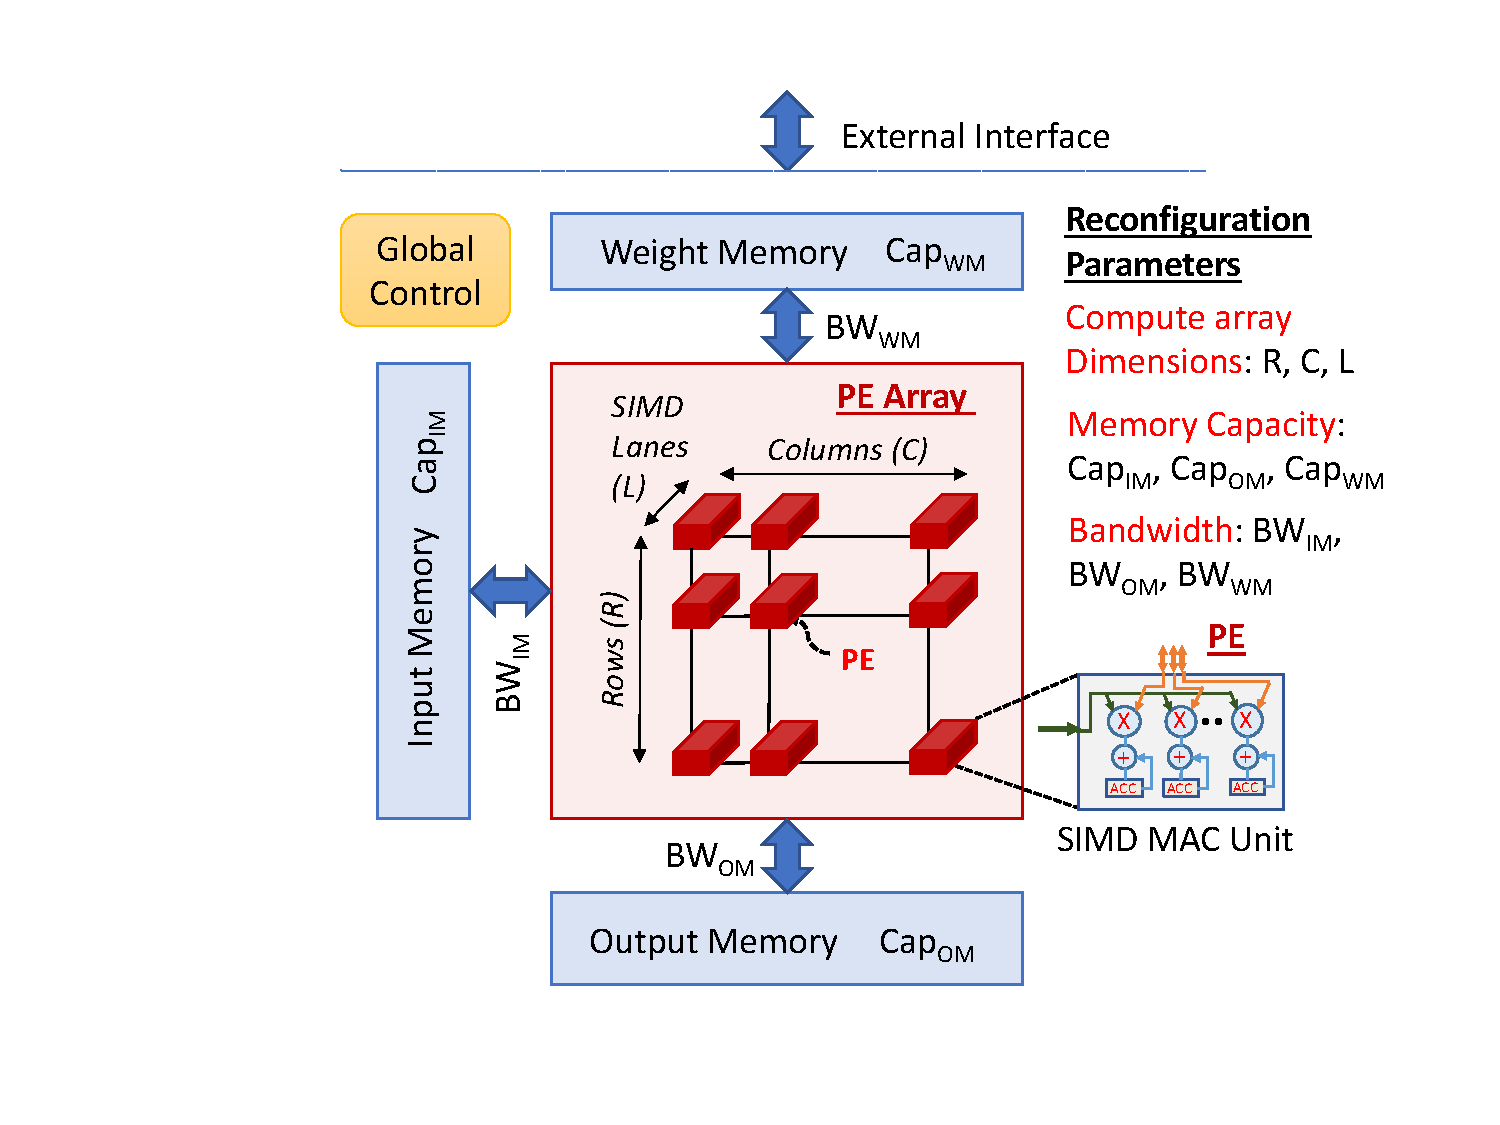
\includegraphics[width=0.8\columnwidth]{fig/syst-array.pdf}
    \caption{A SIMD 2D systolic array accelerator}
    \label{fig:systolic_array}
\end{figure}

To realize convolution and matrix-vector multiplication, we adopt an output stationary dataflow.
In this case, the input is fed along the rows, and the weights are fed along the columns.
The partial sums are accumulated within the PEs, and are further accumulated diagonally before being stored in the output memory.
Specifically, the $\Nij$, $\Kij$ and $\Nout$ workload dimensions are mapped spatially to the rows ($R$), columns ($C$) and SIMD lanes ($L$) of the PE array, while the $\Nin$ dimension is sequenced temporally.

\subsection{General Optimization of DNN acceleration with Reconfigurable Spatial Architectures}

\section{Summary and Plan of Work}

My past research efforts have completed the following work:

\begin{itemize}
    \item Evaluation of hierarchical temporal memory performance and scalability in von Neumann architecture, design and implementation of hierarchical temporal memory in the Automata processor, and evaluation of speedup and scalability in comparison.
    \item Development of a methodology for synthesis, simulation, and validation of hierarchical temporal memory models in the automata processor
\end{itemize}

The following tasks have yet to be completed:

\begin{itemize}
    \item Document and open-source Krycek toolchain for evaluation of DNN workloads on spatial architectures
\end{itemize}

The expected main chapters of my dissertation are:

\begin{itemize}
    \item Mapping hierarchical temporal memory on the Automata processor
    \item Synthesis, simulation, and validation of hierarchical temporal memory in the Automata processor
    \item Optimization of deep neural networks on spatial processor architectures
\end{itemize}